\subsection{Builder (生成器)}
\noindent\textbf{意图}

将一个复杂对象的构建与表示分离,使得同样的构建过程可以创建不同的表示。

\noindent\textbf{动机}

假设我们要实例化一个机器人对象,机器人有手,眼睛,传感器等等参数需要构造。对于不同的机器人有些参数是必要的,有些是不必要的,有些可以使用默认参数。为了实现机器人对象的实例化,我们的构造方法往往会十分复杂,需要加入很多参数,甚至于需要书写不止一个构造函数。

为了避免上述情况,我们可以在机器人内部创建一个 builder 对象,调用 builder 对象不同的方法用于设置不同的参数。在机器人的构造函数中使用 builder 来对这些参数进行赋值\footnote{比较抽象,建议结合例子链接理解。}。因此,含有 builder 的类实例化代码往往是这样的:

\begin{Java}
CompanyClient client = new CompanyClient.Builder()
    .setCompanyName("百度")
    .setCompanyAddress("海定区百度大厦")
    .setCompanyRegfunds(5)
    .setmPerson("1000人以上")
    .build();
\end{Java}

在上述代码中,我们可以有选择性地为 company 设置属性,这样设置属性地方式更加灵活。其中 company 通常被称为导向器(director)。

\noindent\textbf{适用性}

以下情况使用 Builder 模式:
\begin{itemize}
    \item 当创建复杂对象地算法应该独立于该对象地组成部分以及它们地装配方式时。
    \item 当构造过程必须允许被构造的对象有不同的表示时。
\end{itemize}

\noindent\textbf{结构}

Builder 模式的结构如下图所示

\begin{figure}[H]
    \scriptsize
    \centering
    \begin{tikzpicture}[scale = 1]
        \begin{class}[text width=2cm]{Director}{0,-0.2}
            \operation{Construct()}
        \end{class}
        \begin{interface}[text width=2cm]{Builder}{5,0}
            \operation{BuildPart()}
        \end{interface}
        \begin{class}[text width=2cm]{Product}{9,-3.2}
        \end{class}
        \begin{class}[text width=2cm]{ConcreteBuilder}{5,-3}
            \implement{Builder}
            \operation{BuildPart()}
            \operation{GetResult()}
        \end{class}
        \aggregation{Director}{builder}{1}{Builder}
        \draw[umlcd style,->] (ConcreteBuilder) -- (Product);
    \end{tikzpicture}
\end{figure}

\noindent\textbf{参与者}

\begin{itemize}
    \item \textbf{Builder}: 为创建一个 Product 对象的各个部件指定抽象接口。
    \item \textbf{ConcreteBuilder}: 实现接口以构造和装配该产品的各个部件。
    \item \textbf{Director}: 构造一个使用 Builder 接口的对象。
    \item \textbf{Product}: 被构造的复杂对象。
\end{itemize}

\noindent\textbf{协作}
\begin{itemize}
    \item 用户创建 Director 对象,并用他所想要的 Builder 对象进行配置。
    \item 一旦生成了产品部件,导向器就会通知生成器。
    \item 生成器处理导向器的请求,并将部件添加到该产品中。
    \item 客户从生成器中检索产品。
\end{itemize}

下图的交互说明了 Builder 和 Director 是如何与一个客户协作的。

\begin{figure}[H] 
    \centering 
    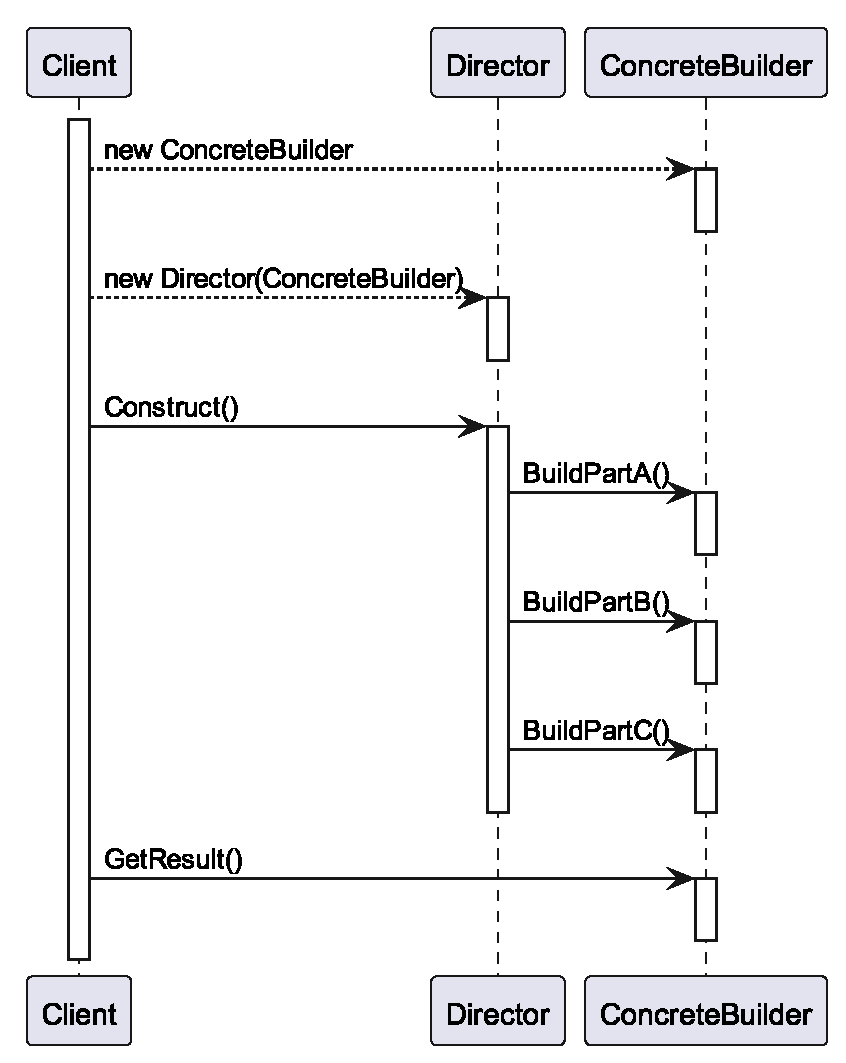
\includegraphics[width=8cm]{figures/Builder.eps} 
\end{figure}

\noindent\textbf{优缺点}
\begin{itemize}
    \item \textbf{可以改变一个产品的内部表示}
    \item \textbf{对构造过程进行更精细的控制}
    \item \textbf{构造代码变得更加复杂,并不美观}
\end{itemize}

\noindent\textbf{实现}
\begin{itemize}
    \item \textbf{装配和构造接口}: 生成器逐步地构造他们的产品。因此 Builder 类接口必须足够普遍,以便为各种类型的具体生成器构造产品。
\end{itemize}

\noindent\textbf{相关模式}
\begin{itemize}
    \item Abstract Factory: 与 Builder 类似,不过 Abstract Factory 注重于多个系列地产品对象。Builder 注重于一步步构造一个复杂的对象。
    \item Composite: 通常用 Builder 生成。
\end{itemize}

\noindent\textbf{例子}
\begin{itemize}
    \item Java 实现 Builder 设计模式: \url{https://blog.csdn.net/qq_17678217/article/details/86507693} 
\end{itemize}

\lstinputlisting[language=Python]{../../scripts/creational/Builder.py}

\newpage